% ********************************* HEADERS ***********************************
\documentclass{article}
% setcounter{secnumdepth}{5}
\usepackage[top=.75in, bottom=.75in, left=.50in,right=.50in]{geometry}
\usepackage{fancyhdr}
\usepackage{titling}
\pagestyle{fancy}
\lhead{EECS 281 - Data Structures and Algorithms}
\rhead{\thepage}
\usepackage{color}
\usepackage{graphicx}
\newcommand{\heart}{\ensuremath\heartsuit}
\usepackage{listings}
\lstset{
  % language=C++,
  showstringspaces=false,
  basicstyle={\small\ttfamily},
  numberstyle=\tiny\color{gray},
  keywordstyle=\color{blue},
  commentstyle=\color{dkgreen},
  stringstyle=\color{dkgreen},
}
\usepackage[colorlinks,urlcolor={blue}]{hyperref}
%\setlength{\parskip}{1em}
\usepackage{parskip}
\usepackage{indentfirst}
\setlength{\droptitle}{-4em}
% \usepackage{concmath}
% \usepackage[T1]{fontenc}
\renewcommand{\theenumi}{\Alph{enumi}}
% ********************************* HEADERS ***********************************
\pagenumbering{gobble}
\begin{document}
\title{\textbf{EECS 281 Lab 8 - Fragmented Data Structures (part 2)}}
\author{Due Tuesday, March 15th, 2017 at 11:59pm}
\date{}
\maketitle
\fancypagestyle{firststyle}
{
   \fancyfoot[L]{Written by Aaryaman Sagar for EECS 281 @ The University of
                 Michigan - Ann Arbor}
   \pagestyle{empty}
}
\thispagestyle{firststyle}

In this lab you will be using the transparent linked list from last lab to
finish writing a memory allocator to allocate memory on the heap!

\section{An untyped memory allocator}
You will be using the transparent list class you wrote in the previous lab to
write an untyped memory allocator very much like the C \texttt{malloc()}
function to allocate memory on the heap.

Memory allocators including the C++ \texttt{new} operator get memory on the
heap through function calls to the operating system.  Your allocator will
track the memory available from all previous requests to the operating system
in a fragmented linked list.

A fragmented data structure is one that comprises of elements stored
discontinuously and possibly of different sizes.  The below two pictures
illustrate the difference between fragmented and non-fragmented data
structures.

\begin{figure}[!htb]
\centering
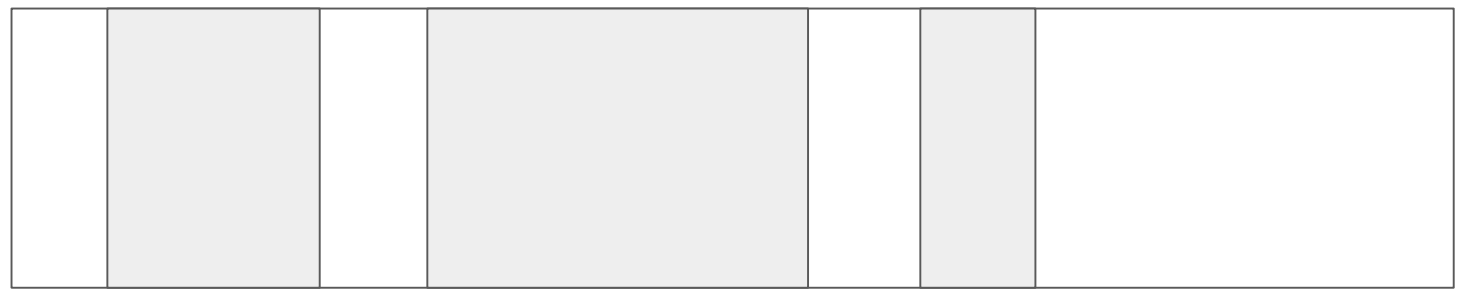
\includegraphics[height=2cm]{fragmented_memory}
\caption{Fragemented memory}
\end{figure}

\begin{figure}[!htb]
\centering
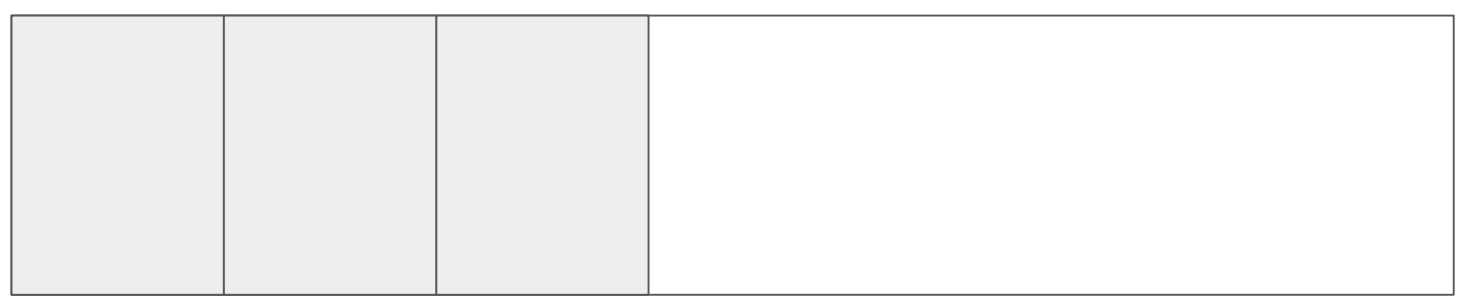
\includegraphics[height=2cm]{non_fragmented_memory}
\caption{Non fragemented memory}
\end{figure}

A memory request is served by returning a block of memory to the user as a
\texttt{void*} pointer.  This allocated memory that is large enough to store
the amount of data the user has asked for.  The allocator keeps track of the
memory segments and how large each segment is by storing a header with the
size information just before the actual usable memory.  The memory map looks
like this, with the black rectangles denoting the headers and the grey the
actual memory blocks.

\begin{figure}[!htb]
\centering
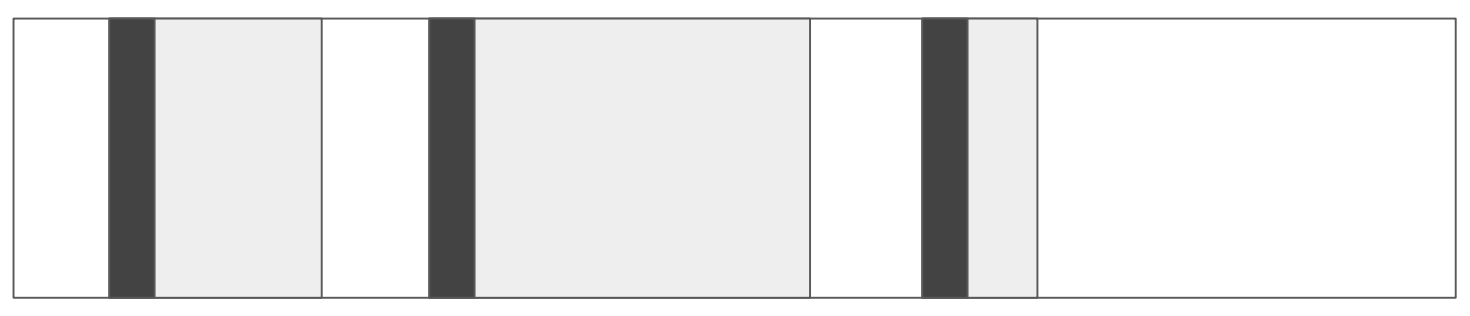
\includegraphics[height=2cm]{memory_storage}
\caption{Memory storage}
\end{figure}

In the above image, the pointer that will be returned to the user for usage
will start at the starting location of the grey area, and the header right
before that will contain the length of that grey area.  This way the allocator
knows how much memory each allocated block points to, so that if the
\texttt{free()} function is called on that memory, it can be put back into the
linked list of headers.

The linked list of headers will resemble the list shown in figure 4 below,
with each header pointing to the next header in the logically increasing order
or addresses (for example here the first header on the left is at a lower
location in memory as compared to the second and the third while the second
one is at a lower location in memory as compared to the third)

\begin{figure}[!htb]
\centering
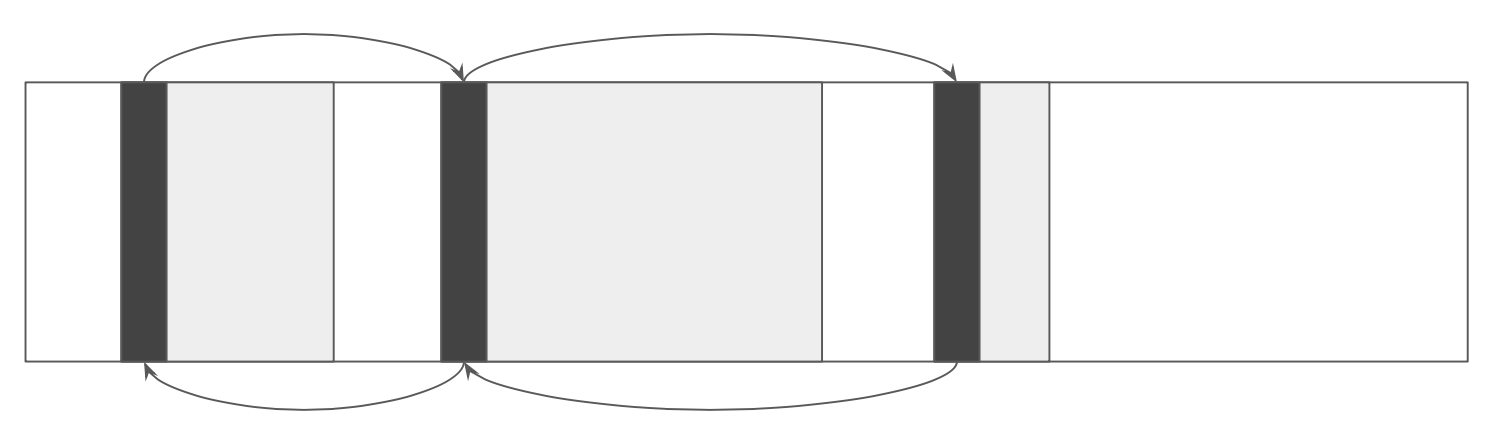
\includegraphics[height=3cm]{linked_list_headers}
\caption{Linked list headers}
\end{figure}

When the user asks for memory, the block with the right amount of memory will
be taken out of the linked list and returned to the user, so for example if
the user asked for a really large portion of memory then the allocator can
return a portion of the second segment to the user.  Subsequently the free
list will be updated to look like so, with the user using the memory in red.

\begin{figure}[!htb]
\centering
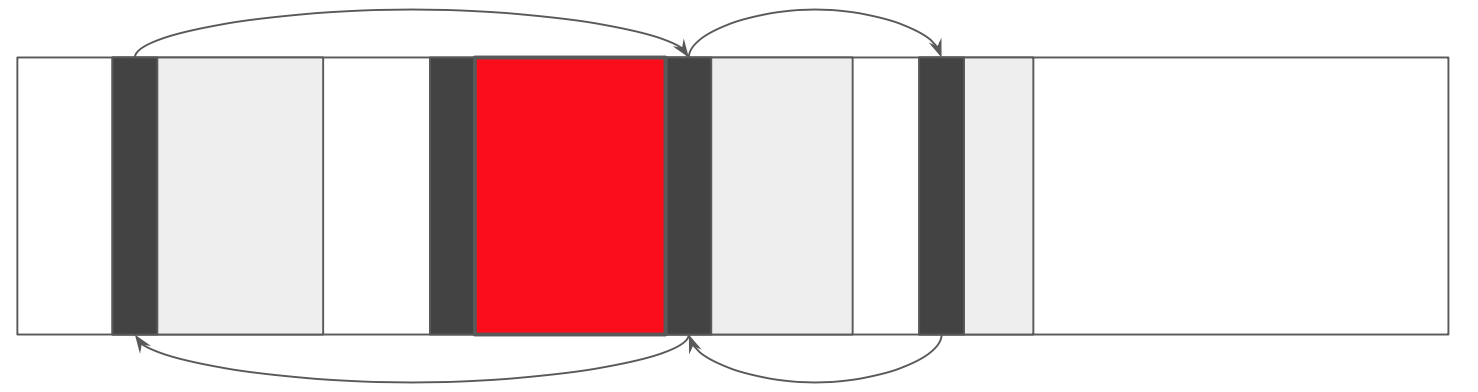
\includegraphics[height=3cm]{after_allocation}
\caption{After an allocation}
\end{figure}

When a user program wants to deallocate the same memory (like a call to
delete) they have to pass the pointer that was allocated via the
\texttt{malloc()} call to \texttt{free()}.  The free function is supposed to
backtrack from the pointer the user passed (which will be pointing to the
beginning of the allocated segment, i.e.  the grey area) back to the header
and put the header back into the linked list.  This can be done via a simple
pointer cast to the header type and decrement by one.  Analagously if you
wanted to get the location of an object of type \texttt{int} right before a
pointer \texttt{ptr}, you would do

\begin{lstlisting}
int* pointer_right_before = static_cast<int*>(ptr) - 1;
\end{lstlisting}

The free function will coalesce memory blocks if they are right by each other
into one bigger block to save on memory used to store headers.  This can be
done through a call to \texttt{coalesce()}.  If the two headers can be
coalesced then the function will coalesce them and return a pointer to the
coalesced header, the function returns a \texttt{nullptr} to denote failure.

\begin{figure}[!htb]
\centering
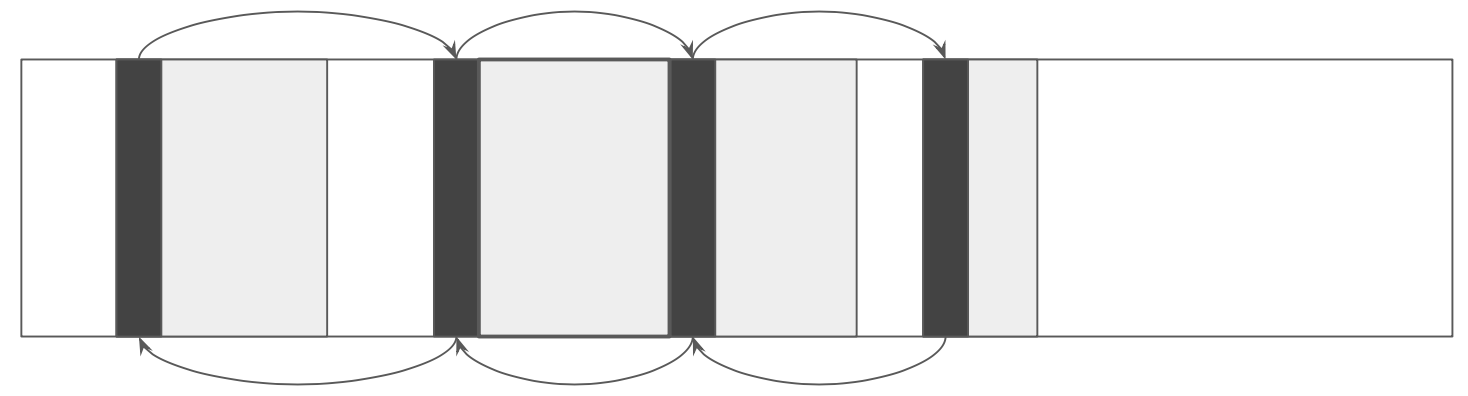
\includegraphics[height=2.3cm]{before_coalescing}
\caption{After a deallocation (before coalescing)}
\end{figure}

\begin{figure}[!htb]
\centering
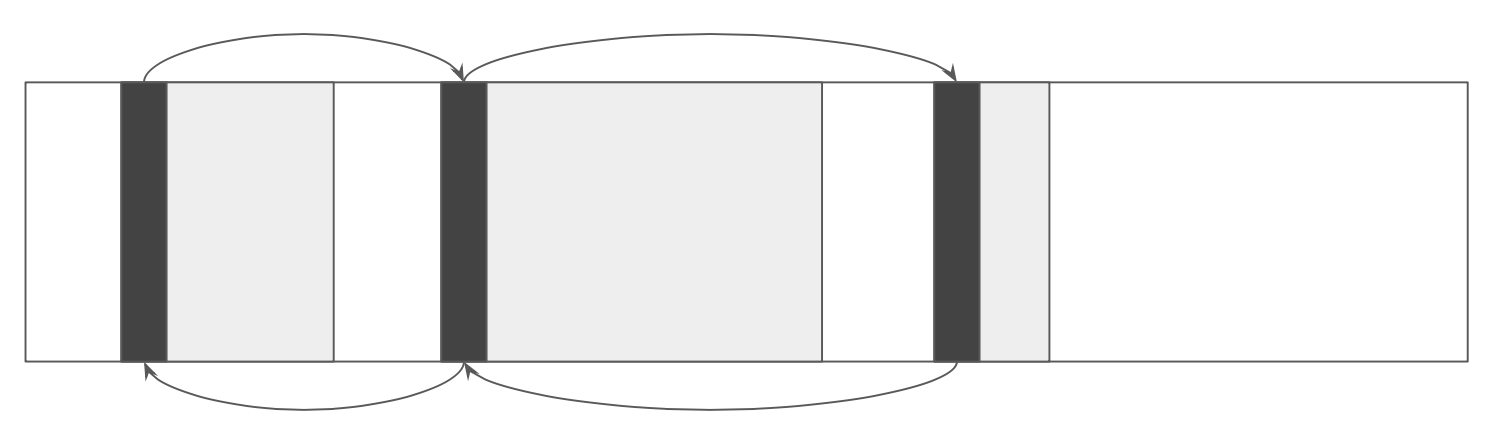
\includegraphics[height=2.3cm]{after_deallocation}
\caption{After a deallocation (after coalescing)}
\end{figure}

\newpage
\subsection{Implementation}
You will be given two modules, one containing the
code and declarations for \texttt{malloc()}, one for the interface to interact
with the operating system and the last one will be your linked list
implementation.  Each will be a pair of a header file and an implementation
file.  You will fill in code in the \texttt{eecs281malloc.cpp} file in the
functions with the \texttt{TODO} symbols.

\subsubsection{\texttt{malloc()}}
All pointers returned via an untyped allocator have to be aligned to the
maximum alignment on the system.  Therefore, the first thing malloc should do
is to align the \texttt{amount} to the max alignment on the system via a call
\texttt{round\_up\_to\_max\_alignment()}.

Then the \texttt{malloc()} function should find the first block with a memory
segment that is large enough to serve the user's request.  This is called a
"first fit algorithm".  If there is no block with a memory segment large
enough to serve the user's request, \texttt{malloc()} will call
\texttt{extend\_heap(int)} with a parameter that is a sum of the aligned
amount variable and the size of a header.  You can get the sizeof a header by
calling \texttt{sizeof(Header\_t)}, after calling \texttt{extend\_heap()}, you
need to construct a header in the location returned by the call to
\texttt{extend\_heap()} by calling \texttt{make\_header()}.  At this point the
free list will have a header that is big enough to serve the user's request.
Insert that header into the linked list after taking out the require memory
via a call to \texttt{remove\_memory()} and then return the pointer to the
user.

It might be useful to use the \texttt{std::find\_if()} algorithm with a custom
functor or lambda function that captures the value of the amount that the user
has asked for.  Another function that might be useful to insert a node into
the linked list in a sorted manner is \texttt{insert\_sorted()}.  As such it's
implementation has been left empty for you to fill and use.

\subsubsection{\texttt{free()}}
The user program must call free for every pointer that it has allocated with
\texttt{malloc()} before terminating the program to avoid memory leaks.  The
\texttt{free()} function puts the memory back in the free list to avoid
repeated calls to the operating system.

The first thing to be done is to fetch a pointer to the header object right
before the pointer passed to \texttt{free()} by the user.  If the user passes
a pointer to memory that has not been returned by a previous call to
\texttt{malloc()} then the behavior is undefined.  To get a pointer to the
header right before the memory allocated by new one would need to cast the
address to a pointer type and then subtract one from it
\begin{lstlisting}
Header_t* header = static_cast<Header_t*>(address) - 1;
\end{lstlisting}

A function called \texttt{coalesce()} should be provided to you declared and
defined in an anonymous namespace.  This function coalesces two headers into
one if they are right after each other in the memory map with nothing in
between.  If the coalescing is not possible, then this function returns a
nullptr and does not modify the contents in either header.  After every call
to \texttt{free()} you have to ensure that all blocks that are coalscable are
coalesced.

\subsection{Appendix}
Free functions that are private to an implementation (\texttt{.cpp}) file file
are generally either put in an anonymous namespace or declared to be static,
both achieve the same effect.
\begin{lstlisting}
static void helper_function() { ... }
namespace {
    void helper_function() { ... }
}
\end{lstlisting}

And the C++ standard favors neither as a superior alternative, this lab uses
the anonymous namespace pattern and as such all "helper" functions are put in
an anonymous namespace.  Therefore when you define helper functions put their
declarations and definitions in an anonymous namespace.


\end{document}


